\documentclass{article}
\usepackage{nips10submit_e,times}

\usepackage{wrapfig}
\usepackage{graphicx}
\usepackage{amsmath,amsthm,amssymb}
\usepackage{natbib}
\usepackage{url}
\usepackage{color}


\newcommand{\mc}{\multicolumn}

\newenvironment{proofof}[1]{\begin{proof}[Proof of #1]}{\end{proof}}

\newenvironment{definition}[1][Definition]{\begin{trivlist}
\item[\hskip \labelsep {\bfseries #1}]}{\end{trivlist}}

\def\thmcolon{\hspace{-.85em} {\bf :} }

\newcommand{\sk}[1]{{\noindent{\textcolor{magenta}{\{{\bf SK:} \em #1\}}}}}

\definecolor{mypurple}{rgb}{.3,0,.5}
\newcommand{\dpf}[1]{\noindent{\textcolor{mypurple}{\{{\bf dpf:} \em #1\}}}}
\newcommand{\note}[1]{\noindent{\textcolor{red}{\{{\bf NOTE:} \em #1\}}}}

%formatting
%\newlength{\IncreaseSpace}
%\setlength{\IncreaseSpace}{0.1in}
%\renewcommand{\baselinestretch}{0.95}

\newcommand{\calL}{\mathcal{L}} 

\newcommand{\eps}{{\epsilon}} 
\newcommand{\argmax}{{\rm argmax}} 
\newcommand{\argmin}{{\rm argmin}} 
\newcommand{\Expct}{{\mathbb E}}
\newcommand{\E}{{\mathbb E}}

\newcommand{\calX}{\mathcal{X}} 

\newcommand{\Xone}{X^{(1)}} 
\newcommand{\Xtwo}{X^{(2)}}
\newcommand{\Xonetwo}{(\Xone,\Xtwo)}

\newcommand{\betatrue}{\beta} 
\newcommand{\betad}{\beta_d} 
%\newcommand{\betaa}{\beta_a} 
%\newcommand{\betab}{\beta_b}

\newcommand{\betas}{\beta_s} 
\newcommand{\betat}{\beta_t} 
\newcommand{\hatbeta}{\hat{\beta}}
\newcommand{\hatbetas}{\hat{\beta}_s}
\newcommand{\hatbetat}{\hat{\beta}_t}

\newcommand{\betaS}{\beta_\mathcal{S}} 

\newcommand{\betabmle}{\hat \betab^{\textrm{MLE}}}


\newcommand{\Projd}{\Pi_d}
%\newcommand{\Proja}{\Pi_a}
%\newcommand{\Projb}{\Pi_b}

\newcommand{\Projs}{\Pi_s}
\newcommand{\Projt}{\Pi_t}

\newcommand{\ProjPCAd}{P_d}
%\newcommand{\ProjPCAa}{P_a}
%\newcommand{\ProjPCAb}{P_b}
%\newcommand{\ProjPCAab}{P_{a,b}}

\newcommand{\ProjPCAs}{P_s}
\newcommand{\ProjPCAt}{P_t}
\newcommand{\ProjPCAst}{P_{s,t}}


\newcommand{\ProjPCASt}{P_{\mathcal{S},t}}

\newcommand{\PCAd}{\mathcal{X}_d}
%\newcommand{\PCAa}{\mathcal{X}_a}
%\newcommand{\PCAb}{\mathcal{X}_b}

\newcommand{\PCAs}{\mathcal{X}_s}
\newcommand{\PCAt}{\mathcal{X}_t}
\newcommand{\PCAsp}{\mathcal{X}_{s,\perp}}
\newcommand{\PCAtp}{\mathcal{X}_{t,\perp}}

\newcommand{\PCAshared}{\mathcal{X}_{s,t}}
\newcommand{\SharedSub}{\mathcal{X}_{\textrm{shared}}}


%\newcommand{\Matob}{{{M}}_{a\rightarrow b}}
%\newcommand{\isoMatob}{\tilde M_{a\rightarrow b}}

\newcommand{\Mstot}{{{M}}_{s\rightarrow t}}
\newcommand{\isoMstot}{\tilde M_{s\rightarrow t}}

\newcommand{\MStot}{{{M}}_{\mathcal{S}\rightarrow t}}

\newcommand{\Mttos}{M_{t\rightarrow s}}
\newcommand{\isoMttos}{\tilde M_{t\rightarrow s}}

\newcommand{\Covs}{\Sigma_{s}}
\newcommand{\Covt}{\Sigma_{t}}
\newcommand{\Covstot}{\Sigma_{s\rightarrow t}}
\newcommand{\CovS}{\widehat{\Sigma}_{\mathcal{S}}}

\newcommand{\Mttod}{M_{t\rightarrow d}}

\newcommand{\xst}{{[x]_{s,t}}}
\newcommand{\xsp}{{[x]_{s,\perp}}}
\newcommand{\xtp}{{[x]_{t,\perp}}}


\newtheorem{theorem}{Theorem}
\newtheorem{lemma}[theorem]{Lemma}
\newtheorem{assumption}[theorem]{Assumption}
\newtheorem{proposition}[theorem]{Proposition}
\newtheorem{corollary}[theorem]{Corollary}
\newtheorem{example}{Example}
\newtheorem{remark}{Remark}

\title{Domain Adaptation with Coupled Subspaces}

\author{
John Blitzer \\
Department of Electrical Engineering and Computer Science\\
University of California, Berkeley\\
Berkeley, CA 94709 \\
\texttt{blitzer@cs.berkeley.edu}\\
\And
Dean Foster and Sham Kakade \\
Department of Statistics \\
University of Pennsylvania \\
\texttt{sham@stat.upenn.edu} \\
}

% The \author macro works with any number of authors. There are two commands
% used to separate the names and addresses of multiple authors: \And and \AND.
%
% Using \And between authors leaves it to \LaTeX{} to determine where to break
% the lines. Using \AND forces a linebreak at that point. So, if \LaTeX{}
% puts 3 of 4 authors names on the first line, and the last on the second
% line, try using \AND instead of \And before the third author name.

\newcommand{\fix}{\marginpar{FIX}}
\newcommand{\new}{\marginpar{NEW}}

\begin{document}

\maketitle

\begin{abstract}
  Domain adaptation algorithms address a key issue in applied machine
  learning: How can we train a system under a \emph{source}
  distribution but achieve high performance under a different
  \emph{target} distribution?  We tackle this question for divergent
  distributions where crucial predictive target features may not even
  have support under the source distribution.  The key intuition we
  formalize is how to link the learning of weights for these
  target-specific features to source features via a coupled subspace.
  We formalize the assumptions under which such coupled learning is
  possible and give finite sample target error bounds (using only
  source training data).  Our algorithm yields good performance on two
  natural language processing adaptation data sets which are
  characterized by the presence of novel features.
\end{abstract}

\section{Introduction}
\label{sec:intro}
% don't use words: alig, zero-shot algo

The supervised learning paradigm of training and testing on identical
distributions has provided a powerful abstraction for developing and
analyzing learning algorithms.  In many natural applications, though,
we train our algorithm on a source distribution, but we desire high
performance on target distributions which differ from that
source~\cite{huang07,xue08,blitzer08,mansour09}.  This is the
problem of domain adaptation, which plays a central role in fields
such as speech recognition~\cite{legetter95}, computational
biology~\cite{liu08}, natural language
processing~\cite{blitzer06,daume07,guo09}, and web
search~\cite{chen08,gao09}.\footnote{Jiang~\cite{JiangReview} provides
  a good overview of domain adaptation settings and models}

In this paper, we address a domain adaptation setting that is common
in the natural language processing literature.  Our target domain
contains crucial predictive features such as words or phrases that do
not have support under the source distribution.
Figure~\ref{fig:examples} shows two tasks which exemplify this
condition.  The left-hand side is an example of a product review
classification task~\cite{blitzer07,dredze08,mansour09}.  The
instances in this task consist of reviews of different different
products from Amazon.com, together with the rating given to the
product by the reviewer (1-5 stars).  The adaptation task is to build
a regression model (for number of stars) from reviews of one product
type and apply it to another.  In the example shown, the target domain
(kitchen appliances) contains phrases like \emph{a breeze} which are
positive predictors but not present at all in the source domain.

The right-hand side of Figure~\ref{fig:examples} is an example of a
part of speech (PoS) tagging
task~\cite{ratnaparkhi96,blitzer06,huangyates}.  The instances consist
of words and their left and right contexts, together with their tags
(noun, verb, adjective, adverb, etc).\footnote{PoS tagging is often
  treated as a sequence-modeling task, but the error is measured on a
  per-token basis} The adaptation task is to build a tagging model
from annotated Wall Street Journal (WSJ) text and apply it to text of
another genre, such as biomedical abstracts (BIO).  In the example
shown, BIO text contains words like \emph{opioid} that we'd like to
assign tags to, but which are not present in the WSJ.

While at first glance this may seem impossible, there is a body of
empirical work achieving good performance in this setting, by coupling
the learning of these novel features to those features which are
shared across domains~\cite{blitzer06,guo09,huangyates}. For example,
in the sentiment data set, the phrase \emph{a breeze} may co-occur
with the words \emph{excellent} and \emph{good} and the phrase
\emph{highly recommended}.  Since these words are also used to express
positive sentiment about books, we can build a representation from
unlabeled target data which couples the weight for \emph{a breeze}
with the weights for these features.


In this work, we formalize assumptions that provably permit the design
of algorithms for domain adaptation, which: 1) allow for transferring
an accurate classifier from our source domain to an accurate
classifier on the target domain and 2) are capable of using novel
features from the target domain.  Based on these assumptions, we give
a simple algorithm that builds a coupled linear subspace from
unlabeled (source and target) data.  We also give finite target error
bounds (using only source training data or a mix of source and target
training data) that depend on how the covariance structure of the
coupled subspace relates to novel features in the target distribution
(which we precisely specify).

\iffalse
Our goal in this work is to formalize the assumptions under which
learning a representation from unlabeled data can allow us to build a
model on the source domain that automatically performs well on the
target.  Bases on these assumptions, we give a simple algorithm that
builds a shared linear subspace from unlabeled source and target data.
We also give finite source-sample target error bounds for our
algorithm that depend on the covariance structure of the shared
subspace under the source and target distributions.  
subspace under the source and target distributions.  Our bound is
similar in spirit to both sample selection bias correction
work~\cite{heckman79,huang07,cortes08} as well as theoretical analyses
of domain adaptation~\cite{blitzer08,mansour09}.  It differs from the
former by accomadating source and target distributions which don't
share support and from the latter by giving rates which asymptotically
approach 0, even when the distributions diverge on the shared
subspace.
\fi

Our work differs from previous treatment of the domain adaptation
setting~\cite{JiangReview} in that we focus on the issue of how to
make use of novel features in the target domain.  Our bound is similar
in spirit to both sample selection bias correction
work~\cite{heckman79,huang07,cortes08} and recent theoretical analyses
of domain adaptation~\cite{blitzer08,mansour09}.  It differs from the
former by accommodating source and target distributions which don't
share support and from the latter by giving rates which asymptotically
approach 0, even when the distributions diverge on the coupled
subspace.

We demonstrate the performance of our algorithm on the sentiment
classification and part of speech tagging tasks illustrated in
Figure~\ref{fig:examples}.  Our algorithm gives consistent performance
improvements from learning a model on source labeled data and testing
on a different target distribution.  Incorporating small amounts of
target data is trivial under our model, since our representation
automatically incorporates target data along those directions of the
shared subspace where it is needed most.
% We demonstrate improved performance in this setting, as well.

\begin{figure*}
\begin{center}
\begin{tabular}{rlccccc}
           \multicolumn{2}{c}{\large{Sentiment Classification}} & & \multicolumn{4}{c}{\large{Part of Speech Tagging}}\\
\hline 
\\
\multicolumn{2}{c}{\textbf{\textcolor{blue}{Books}}} &  \quad \quad \quad & \multicolumn{4}{c}{\textbf{\textcolor{blue}{Financial News}}} \\
\vspace{-0.1in}\\
Positive: & \emph{packed with \textcolor{blue}{fascinating} info} & & NN & VB & VB & NN\\
Negative: & \emph{\textcolor{blue}{plot} is very \textcolor{blue}{predictable}} & & \emph{funds} & \emph{are} & \emph{attracting} & \emph{\textcolor{blue}{investors}}\\
\\
\multicolumn{2}{c}{\textbf{\textcolor{red}{Kitchen Appliances}}} &  & \multicolumn{4}{c}{\textbf{\textcolor{red}{Biomedical Abstracts}}} \\
\vspace{-0.1in}\\
Positive: & {\emph{\textcolor{red}{a breeze} to clean up}} & & NN & PP & ADJ & NN\\
Negative: & \emph{\textcolor{red}{leaking} on my \textcolor{red}{countertop}} & & \emph{expression} & \emph{of} & \emph{\textcolor{red}{opioid}} & \emph{\textcolor{red}{receptors}}\\
\\
\hline
\end{tabular}
\end{center}
\label{fig:examples}
\caption{Examples from two natural language processing adaptation
  tasks, where the target distributions contain words (in red) that do
  not have support under the source distribution.  Words colored in
  blue and red are unique to the source and target domains,
  respectively.  Sentiment classification is a binary (positive
  vs. negative) classification problem.  Part of speech tagging is a
  sequence labeling task, where NN indicates noun, PP indicates
  preposition, VB indicates verb, etc.}
\end{figure*}



\section{Setting}

Our input $X\in\calX$ are vectors, where $\calX$ is a vector
space. Our output $Y\in\mathbb{R}$.  Each domain $D=d$ defines a joint
distribution $\Pr[X,Y|D=d]$ --- while our theory extends to multiple
domains, we only consider the source domain $D=s$ and target $D=t$.
In the covariate shift model, $\Pr[X|D=d]$ may vary with the domain
$D$, while the conditional distribution $\Pr[Y|X,D=d]$ is not a
function of the domain.  We consider a slight modification of this
setting, under the prevalent assumption that we are working in a high
enough dimensional feature space so that a certain linearity
assumption is appropriate.  Formally, we have:

\begin{assumption} \label{ass:same_task}
(Identical Tasks) Assume there there is a vector $\betatrue$ so that
for $d\in {s,t}$:
\[
\Expct [Y|X,D=d] = \betatrue \cdot X
\]
\end{assumption}

%Roughly speaking, this assumption is an idealization of empirical
%finding that there exists one good \emph{simultaneous} linear predict
%for multiple domains (which we empirically is true).

Now suppose we have a labeled training data $T=\{(x,y)\}$ on the
source domain $s$, and we desire to perform well on our target
domain $t$. Let us examine what is transferred by using the naive
algorithm of simply minimizing the square loss on the source domain.

Roughly speaking, using samples from the source domain
$s$, we can estimate $\beta$ in only those directions in which $X$ varies
on domain $s$. Let us define the subspaces in which the source 
and target inputs vary. To make this precise, define the \emph{principal
  subspace} $\PCAd$ for a domain $d$ as the (lowest dimensional)
subspace of $\calX$ such that $X\in \PCAd$ with probability $1$.

There are three natural subspaces between the source domain $s$ and
target domain $t$; the part which is shared and the parts specific to
each. More precisely, define the shared subspace for two domains $s$
and $t$ as $\PCAshared = \PCAs \cap \PCAt$ (the intersection of the
principal subspaces, which is itself a subspace). We can decompose any
vector $x$ into the vector $x=[x]_{s,t}+ [x]_{s,\perp}+
[x]_{t,\perp}$, where the latter two vectors are the projections of
$x$ which lie off the shared subspace (Our use of the ``$\perp$''
notation is justified since one can choose an inner product space
where these components are orthogonal, though our analysis does not
explicitly assume any inner product space on $\calX$).  We can view the
naive algorithm as fitting three components, $[w]_{s,t}$,
$[w]_{s,\perp}$, and $[w]_{t,\perp}$, where the prediction is of the
form:
\[
[w]_{s,t} \cdot [x]_{s,t}+[w]_{s,\perp} \cdot [x]_{s,\perp}+ [w]_{t,\perp}\cdot [x]_{t,\perp}
\]
Here, with only source data, this would result in an unspecified estimate of
$[w]_{t,\perp}$ as $[x]_{t,\perp}=0$ for $x \in \PCAs$. Furthermore, the naive algorithm would only learn 
weights on $[x]_{s,t}$ (and it is this weight, on what is shared,
which is what transfers to the target domain).

Certainly, without further assumptions, we would not expect to be able
to learn how to utilize $[x]_{t,\perp}$ with only training data from
the source. However, as discussed in the intro, we might hope that
with unlabeled data, we would be able to ``couple''  the learning of
features in $[x]_{t,\perp}$ to those on $[x]_{s,t}$. 

\subsection{Unsupervised Learning and Dimensionality Reduction}

Our second assumption specifies a means by which this coupling may
occur. Given a domain $d$, there are a number of semi-supervised
methods which seek to find a projection to a subspace $\PCAd$, which
loses little predictive information about the target. In fact, much of
the focus on un-(and semi-)supervised dimensionality reduction is on
finding projections of the input space which lose little predictive
power about the target. We idealize this with the following
assumption.

\begin{assumption} \label{ass:dim_red} (Dimensionality Reduction) For
  $d\in\{s,t\}$, assume there is a projection
  operator~\footnote{Recall, that $M$ is a projection operator if $M$
    is a linear and if $M$ is idempotent, i.e.  $M^2x=Mx$} $\Projd$
  and a vector $\betad$ such that
\[
\Expct [Y|X,D=d] = \betad \cdot (\Projd X) \, .
\]
Furthermore, as $\Projt$ need only be specified on $\PCAt$ for this assumption, we can
specify the target projection operator so that $\Projt \xsp = 0$ (for convenience).
\end{assumption}

Implicitly, we assume that $\Projs$ and $\Projt$ can be learned from
unlabeled data, and being able to do so is is crucial to the practical
success of our adaptation algorithm.  Our theory is agnostic to the
details of the specific learning algorithm, though.  Indeed, the
empirical adaptation work that does learn shared representations
covers a whole host of techniques, all of which work well for their
particular task~\cite{blitzer06,guo09,huangyates}.  We discuss our
specific algorithm in further detail in
Section~\ref{subsec:learning_projections}.


%% \section{Constructing the Coupled Representation}
\label{subsec:algorithm}

Our algorithm exploits our assumptions to construct a coupled
representation so that learning on the source will force learning on
the novel part of the target subspace, i.e. on $[x]_{t,\perp}$. Once
we have $\Projs$ and $\Projt$, we fit a linear predictor of the form:
\begin{equation}~\label{eq:coupled}
w_t \Projt x  \ + \  w_s \Projs \xsp
\end{equation}
where $w_t$ and $w_s$ are the parameters.  

We briefly discuss here how to find the projection operators $\Projs$
and $\Projt$ and how to identify the portion of the source $\xsp$ that
is not related to the target.  For finding the projections, we use an
approximation to canonical correlation analysis
(CCA)~\cite{hotelling35} for large-scale, high dimensional
data~\cite{ando07,kakade07,fosterTR}.  CCA is a multiple-view
dimensionality reduction algorithm, so we begin by breaking up each
instance into two views.  For example, in the sentiment task we define
view 1 to be the first half of the document and view 2 to be the
second half.  Then we search for the reduced dimensional subspace of
both views that maximizes the correlation between views across all of
the unlabeled data.  On the target domain, for example, the output of
this procedure are two orthogonal projections $\Projt^{(1)}$ and
$\Projt^{(2)}$ which are also orthogonal to each other.  Now we define
$\Projt = \Projt^{(1)} + \Projt^{(2)}$.

CCA-based representations have been shown to perform well for a
variety of semi-supervised learning
tasks~\cite{ando07,kakade07,fosterTR}, but it is not a contribution of
this work, and a detailed description is beyond our scope.  We
emphasize, though, that the predictor in Equation~\ref{eq:coupled} is
agnostic to the specific dimension reduction algorithm.  The only
requirement is that the resulting representation be predictive as in
Assumption~\ref{ass:dim_red}.  Indeed, the empirical adaptation work
that does learn shared representations all use different dimension
reduction techniques~\cite{blitzer06,guo09,huangyates}.

Finding $\xsp$ exactly can be difficult, since any method for
discovering the subspace exactly may suffer from stability issues in
very high dimensional spaces.  We approximate $\xsp$ by simply
projecting onto just those source-unique features which have no
support in the large target unlabeled data.  In the sentiment task
from Figure~\ref{fig:examples}, for example, the
word \emph{fascinating} is just such a source-unique feature.


\section{Generalization under the Coupled Representation}
\label{sec:generalization}

The idea of the algorithm is to construct a shared representation so
that learning on the source will force learning on the novel part of
the target subspace, e.g. on $[x]_{t,\perp}$. Our algorithm fits a
linear predictor of the form:
\begin{equation}~\label{eq:coupled}
w_t \Projt x  \ + \  w_s \Projs \xsp
\end{equation}
where $w_t$ and $w_s$ are the parameters.  

First, the following lemma shows that this representation is
\emph{sound}, meaning that our shared representation supports optimal
predictions \emph{simultaneously} on both the source and target
domains, with $w_t=\betat$ and $w_s=\betas$.

\begin{lemma}~\label{lemma:coupled}
(Soundness) For $d =s$ and $d=t$, we have that:
\[
\Expct[Y|X,D=d] = \betat \Projt x  \ + \  \betas \Projs \xsp
\]
\end{lemma}

\begin{proof}
First, by our projection assumption,
the optimal predictors are:
\begin{eqnarray*}
\Expct[Y|X,D=s] = \betas \Projs \xst  \ + \ & \betas \Projs \xsp& \ + \ 0 \\
\Expct[Y|X,D=t] = \betat \Projt \xst  \ + \  & 0 & \ + \  \betat \Projt \xtp
\end{eqnarray*}
Now, in our domain adaptation setting
(where $E[Y|X,D=d]$ is linear in $X$), we have must have that the
weights on $x_{s,t}$ agree, so that:
\[
\betas \Projs \xst = \betat \Projt \xst
\]
for all $x$.

For $d=t$, the above clearly holds as $\xsp=0$ for $x \in \PCAt$. For
$d=s$, we have $\Projt x = \Projt \xst +\Projt \xsp = \Projt
\xst$ for $x \in \PCAs$, since $\Projt$ is null on $\xsp$ (as
discussed in Assumption~\ref{ass:dim_red}).
\end{proof}

Now, let us provide a little intuition for this representation, before
formally showing how perfect transfer is possible using only
source data. Note that for our source domain, where $x \in \PCAs$, we
have that $\Projt x = \Projt \xst$ (since $\Projt \xsp =0$, as
explained in Assumption~\ref{ass:dim_red}). Hence, our prediction with
$x$ in the source is of the form:
\[
w_t \Projt \xst  \ + \  w_s \Projs \xsp
\]
Thus, if we seek to use $\xst$ in our prediction, then we \emph{must}
place a non-zero weight on at least some components in $w_t$. However,
now the learned weight $w_t$ could have an effect on all of $\xtp$.

\iffalse
First
note, that $w_t$ is a weight acting on $\Projt x$, and this projection
couples the features in $\xst$ with $\xtp$ --- so that with a nonzero weight
$w_t$, our predictions could vary with $\xtp$.
\fi

Our first theorem specifies when perfect transfer is possible using
only source data (e.g. do we converge to a perfect predictor on the
target domain with a sufficiently large sample on the source
domain). Using the notation, $\Projt \PCAt=\{\Projt x: x\in\PCAt\}$,
we have that $\Projt \PCAt$ is the reduced
dimensional predictive subspace for the target domain. Also, note that
$\Projt \PCAshared$ is the subspace of $\Projt \PCAt$ which is due
to the variation in the shared subspace. Note that $\Projt \PCAshared$ could
actually equal $\Projt \PCAt$. For example, say  $\Projt X$
is simply the one dimensional projection $3X_1+5X_3$, where both $X_1$ and $X_3$ are in $\PCAt$. Now
note that we only need to vary$X_1$ (or just $X_3$ or any
one-dimensional linear combination of them) to cause $3X_1+5X_3$ to
vary. In other words, roughly speaking, as long as the shared features
are appropriately coupled to new features (through $\Projt$)), we will have that $\Projt
\PCAshared = \Projt \PCAt$.

\begin{theorem}
\label{thm:perfect}
(Perfect Transfer) Suppose $\Projt
\PCAshared = \Projt \PCAt$. Then any weight
  vector $(w_t,w_s)$ on the coupled representation which is optimal on
  the source, is also optimal on the target.
\end{theorem}

\begin{proof}
  If $(w_t,w_s)$ provides an optimal prediction on $s$, then this
  uniquely (and correctly) specifies the linear map on
  $\PCAshared$. Hence, $w_t$ is such that $w_t \Projt \xst $ is
  correct for all $x$, e.g. $w_t \Projt \xst = \beta \xst$ (where
  $\beta$ is as defined in Assumption~\ref{ass:same_task}). This
  implies that $w_t$ has been correctly specified in
  $\textrm{dim}(\Projt \PCAshared)$ directions. By assumption, this
  implies that all directions for $w_t$ have been specified, as $\Projt \PCAshared=\Projt \PCAt$
\end{proof}

Our next theorem is on generalization, when we have a finite training
dataset (which could consist of only source samples or a mix of
samples from the source and target). For the theorem, we condition on
the inputs $x$ in our training set (e.g. we work in a fixed design
setting), and denote these by $T_{\textrm{training}}$ (of size
$n$). As in the fixed design setting, the randomization is only over
the $Y$ values for these fixed inputs.  Define the following two
covariance matrices:
\[
\Covt = \E[ \ (\Projt x)(\Projt x)^\top |D=t] , \ \ 
\Covstot = \frac{1}{n} \sum_{x\in T_s} (\Projt x)(\Projt x)^\top
\]
Roughly speaking, $\Covstot$ specifies how the training inputs vary in 
the relevant target directions.

\begin{theorem}~\label{thm:gen} (Generalization) Assume that
  $\mathrm{Var}(Y|X)\leq 1$.  Let: our coordinate system be such that
  $\Covt=I$; $\calL_t(w)$ be the square loss on the target domain; and
  $(\hat w_t,\hat w_s)$ be the empirical risk minimizer with a
  training sample of size $n$. Then our expected regret is:
\[
E[\calL_t(\hat w_t,\hat w_s)] - \calL_t(\beta_t,\beta_s) \leq \frac{\sum_i \frac{1}{\lambda_i}}{n}
\]
where $\lambda_i$ are the eigenvalues of $\Covstot$ and the
expectation is with respect to random samples of $Y$ on the fixed
training inputs.
\end{theorem}

The proof is in Appendix~\ref{app:proof}.  For the above bound to be
meaningful we need the eigenvalues to be nonzero --- this amounts to
having variance in all the directions in $\Projt \PCAt$ (as this is
subspace corresponding to target error covariance matrix
$\Covt$). Note that some target data could greatly reduce the inverse
eigenvalues eigenvalues, thus providing for better generalization.

We briefly compare our bound to the adaptation generalization results
of Ben-David et al.~\cite{ben-david07} and Mansour et
al.~\cite{mansour09colt}.  The bounds they provide bounds factor as an
approximation term that goes to 0 as the amount of source data goes to
infinity and a bias term that depends on the divergence between the
two distributions.  If perfect transfer (Theorem~\ref{thm:perfect}) is
possible, then our bound will converge to 0 without bias.  Note that
Theorem~\ref{thm:perfect} can hold even when there is large divergence
between the source and target domains, as measured by Ben-David et
al.~\cite{ben-david07} and Mansour et al.~\cite{mansour09colt}.  On
the other hand, there may be situations where for finite source
samples our bound is much larger due to small eigenvalues of
$\Covstot$.  Finally we note that if some eigenvalues are $0$ (i.e. we
are missing some relevant directions), then it is possible to include
a bias term for our bound (as a function of $\beta_t$), though due to
space constraints, this is not provided.



\section{Experiments}
\label{sec:experiments}

We evaluate our coupled learning algorithm (Equation~\ref{eq:coupled})
on the sentiment classification and part of speech tagging tasks
illustrated in Figure~\ref{fig:examples}.  The sentiment classification
task~\cite{blitzer07,mansour09,dredze08} consists of reviews of four
different types of products: books, DVDs, electronics, and kitchen
appliances from Amazon.com.  Each review is associated with a rating
(1-5 stars), which we will try to predict.  The smallest product type
(kitchen appliances) contains approximately 6,000 reviews.  The
original feature space of unigrams and bigrams is on average
approximately 100,000 dimensional.  

The part-of-speech tagging data
set~\cite{blitzer06,huangyates,pennbioie} is a much larger data set.
The two domains are articles from the Wall Street Journal (WSJ) and
biomedical abstracts from MEDLINE (BIO).  The task is to annotate
words with one of 39 tags.  For each domain, we have approximately 2.5
million words of raw text (which we use to learn $\Projs$ and
$\Projt$), but the labeling conditions are quite asymmetric.  The WSJ
corpus contains the Penn Treebank corpus of 1 million annotated
words~\cite{penntb}.  The BIO corpus contains only approximately 25
thousand annotated words, however.

We model each word and its part of speech the tag of each word
separately, conditioned on the word and its immediate one-word left
and right context.  As an example context, in
Figure~\ref{fig:examples}, the window around the word \emph{opioid} is
\emph{of} on the left and \emph{receptors} on the right.  The original
feature space consists of these words, along with character prefixes
and suffixes and is approximately 200,000 dimensional.

\subsection{Learning $\Projs$ and $\Projt$}
\label{subsec:learning_projections}

We briefly discuss here how to find the projection operators $\Projs$
and $\Projt$ and how to identify the portion of the source $\xsp$ that
is not related to the target.  For finding the projections, we use an
approximation to canonical correlation analysis
(CCA)~\cite{hotelling35} for large-scale, high dimensional
data~\cite{ando07,kakade07,fosterTR}.  CCA is a multiple-view
dimensionality reduction algorithm, so we begin by breaking up each
instance into two views.  For the sentiment task we define view 1 to
be the first half of the document and view 2 to be the second half.
For the PoS task, we create a two-view representation by dividing up
each segment into content (the word itself) and context (the
surrounding words).

After defining multiple views, we search for the reduced dimensional
subspace of both views that maximizes the correlation between views
across all of the unlabeled data.  On the target domain, the output of
this procedure are two orthogonal projections $\Projt^{(1)}$ and
$\Projt^{(2)}$ which are also orthogonal to each other.  Now we define
$\Projt = \Projt^{(1)} + \Projt^{(2)}$.  In all sentiment experiments,
we set the dimensionality of $\Projs$ and $\Projt$ to be 40.  In all
the PoS tagging experiments, we set the dimensionality of $\Projs$ and
$\Projt$ to be 200 from the context projection and 100 from the
content projection, for a total of 300.

  %% Finally, we note that we concatenate our reduced-dimensional
  %% representation with prefixes and suffixes that are shared across
  %% domains, which allows us to capture morphological cues that may not
  %% be easy to detect from lexical statistics
  %% alone~\cite{ratnaparkhi96}.

Using CCA-induced representations for input to supervised models has
been shown to be useful both theoretically and
empirically~\cite{ando07,kakade07}.  It is not a contribution of this
work, though, and space prevents us from giving a detailed description
of the CCA objective and the specific approximation of Ando and
Zhang~\cite{ando07}, which we use here.  We refer the reader to that
work for details.

We approximate $\xsp$ by simply projecting onto just those
source-unique features which have no support in the large target
unlabeled data.  In the sentiment task from Figure~\ref{fig:examples},
for example, the word \emph{fascinating} is just such a source-unique
feature.

\subsection{Adaptation with Source Only}

\begin{figure}
\hspace{-0.5in}
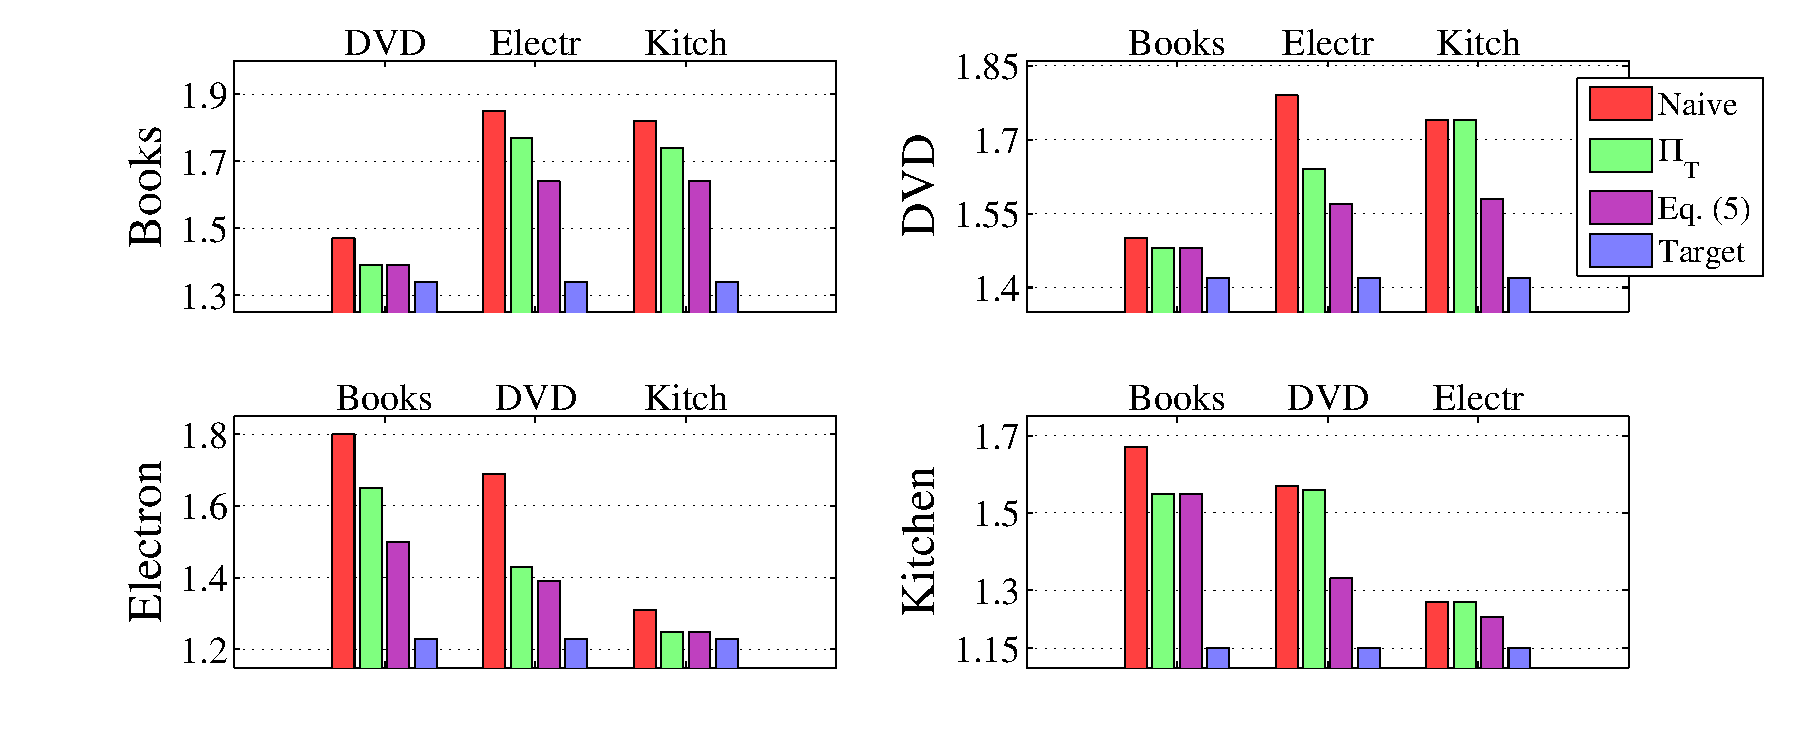
\includegraphics[width=6.4in]{figures/sentiment.pdf}
\vspace{-0.3in}
\caption{Squared error for the sentiment data (1-5 stars).  Each of
  the four graphs shows results for a single target domain, which is
  labeled on the Y-axis.  Clockwise from top left are books, dvds,
  kitchen, and electronics.  Each group of three bars represents one
  pair of domains, and the error bars indicate the standard deviation
  over 10 random draws of source training and target test set.  The
  red bar is the na\"{i}ve algorithm which does not exploit $\Projt$
  or $\Projs$.  The green is our coupled learning algorithm with only
  source data.  The blue (train on target) bars are unaffected by
  source and constant across target domains.}
\label{fig:sentiment_results}
\end{figure}

We begin by evaluating the target performance of our coupled learning
algorithm when learning only from labeled source data.
Figure~\ref{fig:sentiment_results} shows the performance on sentiment
data of the coupled model (in green) versus a na\"{i}ve model (in red)
which simply learns based on the original feature representation,
without taking advantage of projections $\Projt$ and $\Projs$.  The
blue bars train a model directly on the target data and can be thought
of as a ``lower bound'' on error for adaptation.  We defer comparisons
with other adaptation algorithms to Section~\ref{subsec:other}.

\begin{wrapfigure}{l}{3.5in}
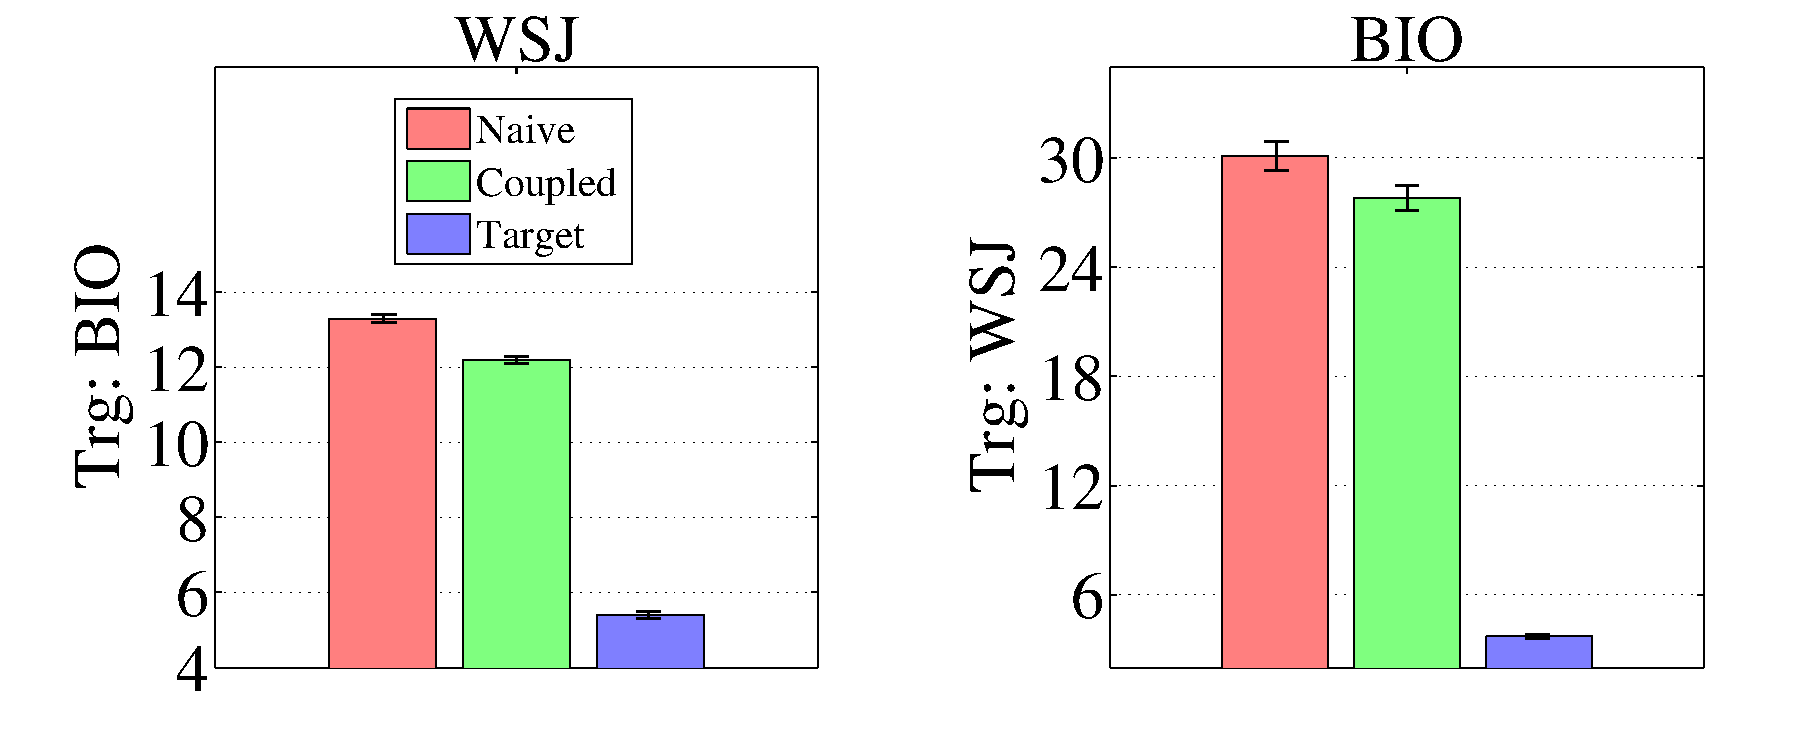
\includegraphics[width=3.5in]{figures/pos.pdf}
\caption{Per-token error for the part of speech tagging task.  Left is from WSJ to BIO.  Right is from BIO to WSJ.  The algorithms are the same as in Figure~\ref{fig:sentiment_results}.}
\label{fig:pos_results}
\end{wrapfigure}

Since we are able to incorporate unseen features via the shared
representation, our theory predicts an improvement in target
performance.  Our algorithm never causes an increase in error and
often greatly improves improves over the na\"{i}ve model.  It is also
worth mentioning that certain pairs of domains overlap less than
others.  For example, books and DVDs are highly overlapping in
vocabulary usage, but books and kitchen appliances are not.  Our
method performs especially well (relative to the baseline) for those
pairs of very dissimilar domains where there are many new,
target-specific features.  We explore this further in
Section~\ref{sec:newnorm}

Figure~\ref{fig:pos_results} illustrates the the coupled learner for
part of speech tagging.  In this case, the variance among experiments
is much smaller due to the larger training data.  Once again, our
method always improves over the na\"{i}ve model.  Finally, we note
that because of data asymmetry, our WSJ models are generally much
better than our BIO models.  In particular, in the right-hand plot,
the BIO source model is trained on only 12,500 words, but the WSJ
target model is trained on 1 million.

\subsection{Adaptation with Source and Target}

\begin{figure}
\hspace{-0.5in}
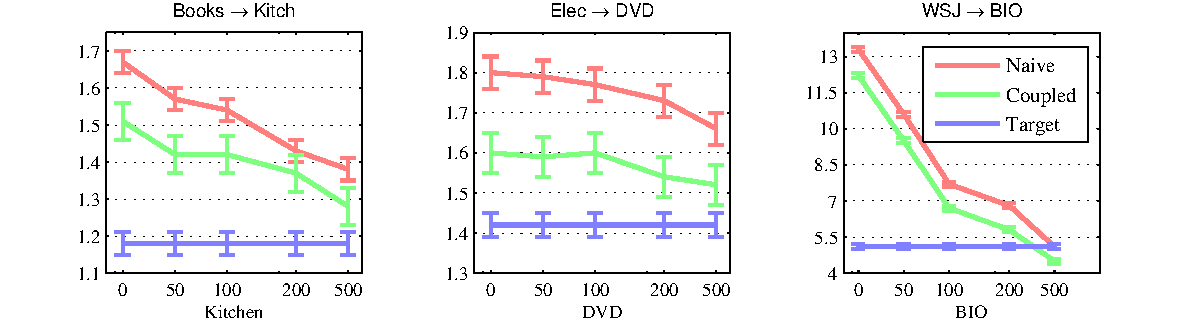
\includegraphics[width=6.5in]{figures/withtarget.pdf}
\caption{Including some target data.  Each figure represents one pair of domains.  The $x$ axis indicates the amount of target data.}
\label{fig:withtarget}
\end{figure}

Our theory indicates that target data can be helpful in stabilizing
predictors learned from the source domain, especially when the domains
diverge somewhat on the shared subspace.  Of course, we also expect
target data to help the na\"{i}ve algorithm as well, but here we show
that our coupled predictors continue to consistently improve over the
naive predictors, even when we do have labeled target training data.
Figure~\ref{fig:withtarget} demonstrates this for three selected
domain pairs.  In the case of part of speech tagging, we use all of
the available target labeled data, and in this case we see a
significant improvement over the target only model (blue curve).
Because of space constraints, we don't show results for all pairs of
domains, but these results are representative.

\subsection{Use of target-specific features}
\label{sec:newnorm}

\begin{figure}
\begin{center}
\begin{tabular}{|c|c|c|}
\hline
\vspace{-0.14in}\\
Adaptation & Negative Target Features & Positive Target Features \\
\hline
\vspace{-0.14in}\\
Books to Kitch & \emph{mush, bad quality, broke,} & \emph{dishwasher, evenly, super easy} \\ 
& \emph{warranty, coffeemaker} & \emph{works great, great product}\\
\hline
\vspace{-0.14in}\\
Kitch to Books & \emph{critique, trite, religious} & \emph{wonderful book, introduction to} \\
& \emph{the publisher, the author} & \emph{illustrations, good reference, relationships} \\
\hline
\end{tabular}
\end{center}
\label{fig:target-specific}
\caption{Illustration of how the coupled learner
  (Equation~\ref{eq:coupled}) uses unique target-specific features for the
  pair of sentiment domains \emph{Books} and \emph{Kitchen}.  We train
  a model using only source data and then find the most positive and
  negative features that are target specific by examining the weights
  under $\left[w_{t}\Projt\right]_{t,\perp}$.}
\end{figure}

Here we briefly explore how the coupled learner puts weight on unseen
features.  One simple test is to measure the relative mass of the
weight vector that is devoted to target-specific features under
different models.  Under the na\"{i}ve model, this is 0.  Under the
shared representation, it is the proportion of $w_{t}\Projt$ devoted
to genuinely unique features.  That is, $\frac{||\left[w_{t}\Projt\right]_{t,\perp}||^{2}_{2}}{||w_{t} \Projt||^{2}_{2}}$.  This quantity
is on average 9.5\% across all sentiment adaptation task pairs and
32\% for part of speech tag adaptation.  A more qualitative way to
observe the use of target specific features is shown in figure
\ref{fig:target-specific}.  Here we selected the top target-specific
words (never observed in the source) that received high weight under
$w_{t}\Projt$.  Intuitively, the ability to assign high weight to
words like \emph{illustrations} when training on only kitchen
appliances can help us generalize better.

\subsection{Validity of Assumptions}

While our theory depends on Assumptions~\ref{ass:same_task} and
\ref{ass:dim_red}, we do not expect them to hold exactly in practice.
Here we examine the extent to which they hold true for our particular
tasks.  The basic idea is to exploit the fact that we do possess
labeled target data for the two data sets to examine source and target
performance under different conditions.  For
Assumption~\ref{ass:same_task}, we compare the performance of a joint
predictor with the performance of a predictor trained on just one
domain.  If these two differ by a small amount, then
Assumption~\ref{ass:same_task} approximately holds.  Training a joint
predictor on books and kitchen appliance reviews together results in a
1.38 mean squared error on books, versus 1.35 if we train a predictor
from books alone.  On kitchen appliances, the joint error is 1.23
versus 1.19 for the individual predictor.  For part-of-speech tagging,
the results are similar: 4.2 joint error versus 3.7 WSJ-only error on
the Wall Street Journal.

For Assumption~\ref{ass:dim_red}, we performed a similar set of
experiments, training with both the reduced-dimensionality
representation (under $\Projd$) and the full feature representation
with all the in-domain training data we had.  For the WSJ, the reduced
dimensional representation achieves 4.2\% error (versus 3.7\% with the
original feature representation).  For DVDs, the reduced-dimensional
representation achieves a 1.47 mean squared error versus a 1.41 mean
squared error for electronics.  For electronics, the
reduced-dimensional representation achieves a 1.23 mean squared error
versus a 1.21 for the full representation.

\subsection{Alternative Adaptation Algorithms}
\label{subsec:other}

Our coupled learning approach performs well for domain adaptation, but
it is not the only algorithm designed for this problems.  Of the
empirical algorithms, the structural correspondence learning work of
Blitzer et al.~\cite{blitzer06} is the most closely-related, but we
note that on the same sentiment data set that algorithm did not give
as consistent gains as ours (and indeed sometimes hurt performance).
The instance weighting algorithms advocated for sample selection bias
correction~\cite{huang07,cortes08} are designed for cases when the
distributions share support and are thus not appropriate for our
setting, but we do note that Jiang and Zhai~\cite{jiang07} report poor
performance using instance weighting for the PoS tagging task.  

When labeled data does exist, there do exist other algorithms that
exploit it by specifically seeking to relax
Assumption~\ref{ass:same_task}~\cite{argyriou07,daume07,finkel09}.
These algorithms do not exploit unlabeled target data, however, and
thus are not directly comparable to our coupled learner.  Indeed, they
are complementary and could potentially give gains when used together
with our coupled representation, although exploration of that is
beyond the scope of this paper.


\section{Conclusion}
\label{sec:conclusion}

Domain adaptation algorithms have been extensively studied in nearly
every field of applied machine learning.  What we formalized here, for
the first time, is how to adapt from source to target when crucial
target features do not have support under the source distribution.
Our formalization leads us to suggest a simple algorithm for
adaptation based on a low-dimensional coupled subspace.  Under natural
assumptions, this algorithm allows us to learn an optimal target
predictor from labeled source data and unlabeled target data.
Furthermore, we show that incorporating small amounts of labeled
target data can improve the stability of our target predictor, both
theoretically and empirically.  We believe our analysis will lead to
interesting connections to other work on adaptation and transfer
learning, especially supervised shared subspace
methods~\cite{argyriou07,daume07}.


\bibliographystyle{plain}
\bibliography{nips2010Transfer}

\newpage
%\pagebreak
\appendix
\section{Appendix}
\label{app:proof}

We now prove Theorem~\ref{thm:gen}.

\begin{proof}
First, note that our expected regret, when $\Sigma_t = I$ is just:
\[
\E \| \hat w_t - \beta_t\|^2
\]
We can also choose our coordinate system so that $\xsp$ is
(statistically) uncorrelated with $\xst$. Then our estimate of $w_t$
is just $ \Covstot^{-1}\widehat \E [(\Projt X) Y]$, where 
\[
\E [(\Projt X) Y] = \frac{1}{n} \sum_{(x,y) \in T} (\Projt x) y
\]
where $(x,y)$ are the values in our training set.  Define $\eta_x$ for
$x$ in our training set by $y_x= \E[Y|x]+\eta_x$, where $y_x$ is the
value on training sample $x$.  By assumption, $\E \eta_x^2 \leq 1$.  If we rotate to a coordinate system where
$\Covstot$ is diagonal, then:
\begin{eqnarray*}
\E \| \hat w_t - \beta_t\|^2 &=& 
\E ||\widehat \E [(\Projt X) Y] - \E [(\Projt X)Y]||_{\Covstot^{-2}}^2\\
& = & \E \left[ \sum_i 
\frac{(\widehat \E [(\Projt X)_i Y] - \E [(\Projt
  X)_iY])^2}{\lambda_i^2}
\right]\\
& = & \E\left[ \sum_i 
\frac{ \left(\frac{1}{n} \sum_{x\in T} \eta_x (\Projt x)_i
  \right)^2}{\lambda_i^2}
\right]\\
& = & \E \left[ \sum_i 
\frac{ \frac{1}{n^2} \sum_{x\in T} \eta_x^2 (\Projt x)_i^2}{\lambda_i^2}
\right]\\
& \leq & \sum_i 
\frac{ \frac{1}{n^2} \sum_{x\in T} (\Projt x)_i^2}{\lambda_i^2}\\
& =& \frac{1}{n} \sum_i 
\frac{ 1}{\lambda_i}
\end{eqnarray*}
where the third to last step uses independence and the final step uses
the definition of $\lambda_i$.
\end{proof}


\end{document}
